\appendix
\section{Segmentation}\label{sec_segmentation_app}

In this chapter, the equations used for placing the wires in the DCH are give. The same naming convention is as well used for the description of the geometry in FCCSW\footnote{\href{https://github.com/HEP-FCC/FCCSW/tree/master/Detector/DetFCCeeIDEA}{https://github.com/HEP-FCC/FCCSW/tree/master/Detector/DetFCCeeIDEA}}. \cref{wires_dch} shows a wire rotated with a stereo angle of $\epsilon$. The angle $\alpha = 30^{\circ}$ remains constant throughout all the layers.


\begin{figure}[ht]
  \begin{subfigure}[b]{0.49\textwidth}
	   \centering
	   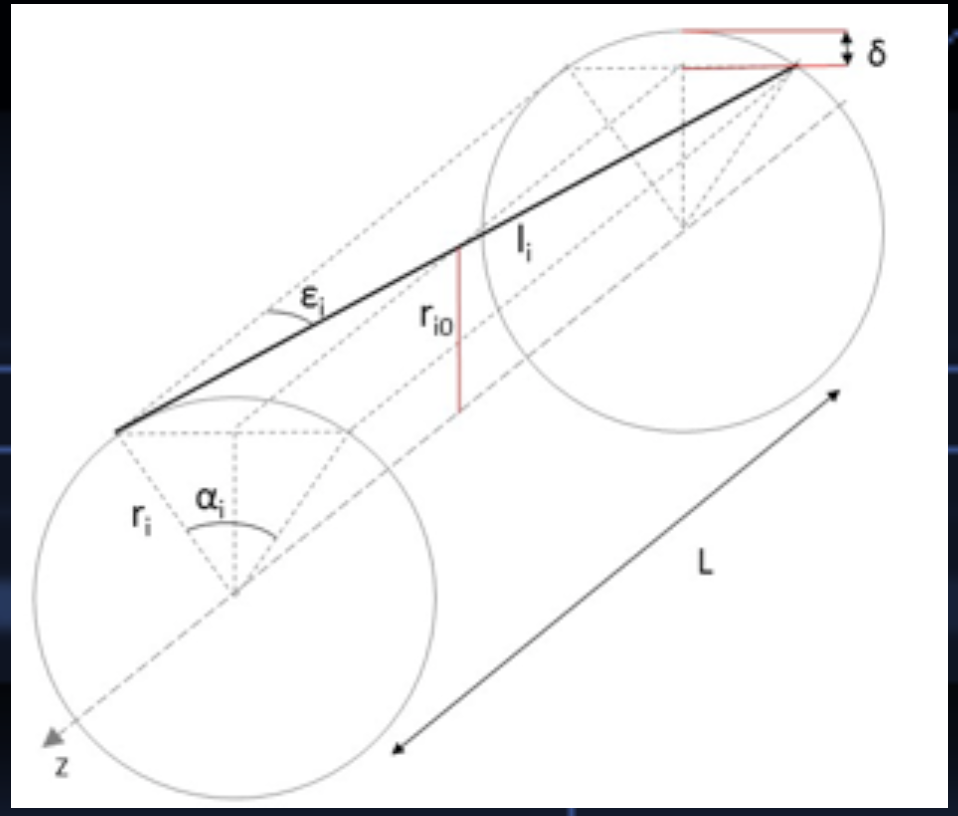
\includegraphics[width=\textwidth]{figures/wires_DCH.png}%
     \caption{}
     \label{fig_wire_3d}
  \end{subfigure}~
  \begin{subfigure}[b]{0.49\textwidth}
	   \centering
     \begin{tikzpicture}[scale=0.8]

       \pgfmathsetmacro{\R}{2}
       \pgfmathsetmacro{\wireAng}{45}

       \coordinate (O) at (0,0);
       \foreach \angle in
       {45,135}
       {
         \fill (\angle:\R) circle (0.1cm);
       }
       \draw (0,0) circle (\R);

       \draw[blue]
       (\wireAng:\R) coordinate (wire1) --
       (3*\wireAng:\R) coordinate (wire2)
       pic [draw,->,angle radius=1cm,"$\alpha$", red] {angle = wire1--O--wire2};

       \draw
       (\R,0) coordinate (xcoord) --
       node[midway,below] {R} (O) --
       (\wireAng:\R) coordinate (slcoord)
       pic [draw,->,angle radius=1cm,"$\phi$"] {angle = xcoord--O--slcoord};

       \draw[-] (O) -- (wire2);

       \node[draw=none, right] at (wire1) {$w_{end}$};
       \node[draw=none, above, blue] at (wire2) {$\Delta a$};
       \node[draw=none, left] at (wire2) {$w_{start}$};

       \begin{scope}[]
         \draw[->] (-2.5,0) -- (2.5,0) node[right] {$x$};
         \draw[->] (0,-2.5) -- (0,2.5) node[above] {$y$};
       \end{scope}
     \end{tikzpicture}
     \caption{}
     \label{fig_wire_2d}
  \end{subfigure}~
	\caption{(a) shows a wire as place in a 3D space and rotated with a stereo angle $\epsilon$. (b) shows the projection of the wire in (a) into the xy-plane. $\alpha$ is the angle between the wire extremities in the xy-plane and it remains the same for all the layers ($\alpha = 30^{\circ}$).}
	\label{wires_dch}
\end{figure}

\cref{eq_a,eq_alpha} give the relationship between $\alpha$ and $\epsilon$ where $L$ is the length of the drift chamber as shown in \cref{fig_wire_3d}.



\begin{equation}
  \Delta a = L \cdot \tan(\epsilon)
  \label{eq_a}
\end{equation}


\begin{equation}
  \alpha = 2 \cdot \arcsin\left({{L \cdot \tan(\epsilon)} \over {2
        \cdot R}}\right)
    \label{eq_alpha}
\end{equation}

\cref{eq_wstart,eq_wend} provide the coordinates of the extremities of the wires depending on the azimuthal angle $\phi$ where $\left|\phi_{start}-\phi_{end}\right| = \alpha$.

\begin{equation}
  \vec{w}_{start} = \begin{pmatrix}
    R \cos(\phi_{start}) \\
    R \sin(\phi_{start}) \\
    L/2
  \end{pmatrix}
  \label{eq_wstart}
\end{equation}

\begin{equation}
  \vec{w}_{end} = \begin{pmatrix}
    R \cos(\phi_{end}) \\
    R \sin(\phi_{end}) \\
    -L/2
  \end{pmatrix}
  \label{eq_wend}
\end{equation}

The distance of the closest approach between a hit position $\vec{p}_{hit}$ and a wire is given by \cref{dist_closest_app}.

\begin{equation}
  d = {{|(\vec{w}_{end}-\vec{w}_{start}) \times
    (\vec{w}_{start}-\vec{p}_{hit}) |} \over {|(\vec{w}_{end}-\vec{w}_{start})|}}
    \label{dist_closest_app}
\end{equation}
